\section{Motivation and Scope}

There has been a strong desire for a more space- and/or runtime-efficient
representation for \code{map} among C++ users for some time now.  This has
motivated discussions among the members of SG14 resulting in a
paper\footnote{See P0038R0,
  \href{http://www.open-std.org/jtc1/sc22/wg21/docs/papers/2015/p0038r0.html}{here}.},
numerous articles and talks, and an implementation in Boost,
\code{boost::container::flat_map}\footnote{Part of Boost.Container,
  \href{http://www.boost.org/doc/libs/1_61_0/doc/html/container.html}{here}.}.
Virtually everyone who makes games, embedded, or system software in C++ uses
the Boost implementation or one that they rolled themselves.\\

Here are some numbers that show why.  The graphs that follow show runtimes for
different \code{map}-like associative containers.  The containers used are
Boost.FlatMap, \code{map}, and two thin wrappers over a sorted \code{vector};
the ``custom pair'' version of the sorted \code{vector} uses a simple
\code{struct} instead of \code{pair} for its value type.  All containers use
an \code{int} as the key type and an \code{int} or a \code{struct} with 5
\code{double}s for the value type.\\

All the graphs below were produced on Windows with MSVC 2015.  Similar results
were obtained on Linux, with Clang 3.9 and libc++, and with g++ 4.8.4 and
libstdc++.\\

These four TODO graphs cover the \code{int}-value-type case.  The first graph
shows insertion of N elements with random keys; the second shows full
iteration across all N elements; the third shows \code{map.find()} called once
for each key used in the original insertions; and the fourth shows erasure of
all N elements, by the keys used in the original insertions.

\begin{tikzpicture}[baseline]
    \begin{groupplot}[group style={group size= 2 by 4}, width=3.25in]

    \nextgroupplot[
        %small,%legend pos=outer north east,legend entries={Boost.FlatMap,std::map,std::unordered\_map,std::vector,std::vector (custom pair)},
        %width=3.75in,
        title={Insert Operations, <int, int> Elements},
        xlabel={N},
        ylabel=\empty,%{Time [milliseconds]},
        xmin=0, xmax=10000,
        ymin=0, ymax=30.0,
        xtick={10,100,1000,10000,100000},
        xticklabels={10,,$10^{3}$,$10^{4}$,$10^{5}$},
        ytick={0.0,10.0,20.0,30.0,40.0},
        ymajorgrids=true,
        grid style=dashed,
        scaled x ticks=false,
        scaled y ticks=true,
        ]

    \addplot[color=blue,mark=|,no markers,]
        coordinates {(10,0.007626)(100,0.0725654)(1000,0.748165)(10000,25.2264)};

    \addplot[color=red,mark=|,no markers,]
        coordinates {(10,0.0070264)(100,0.0703298)(1000,0.612005)(10000,6.07091)};

    \addplot[color=brown,mark=|,no markers,]
        coordinates {(10,0.0082692)(100,0.0839602)(1000,0.65392)(10000,6.22599)};

    \addplot[color=green,mark=|,no markers,]
        coordinates {(10,0.0069982)(100,0.0640582)(1000,0.750933)(10000,23.9862)};

    \addplot[color=black,mark=|,no markers,]
        coordinates {(10,0.006927)(100,0.0595058)(1000,0.628059)(10000,11.1191)};

    \coordinate (top) at (rel axis cs:0,1);% coordinate at top of the first plot

    \nextgroupplot[
        %small,
        %width=3.75in,
        title={Insert Operations, <string, string> Elements},
        xlabel={N},
        ylabel=\empty,%{Time [milliseconds]},
        xmin=0, xmax=10000,
        ymin=0, ymax=400.0,
        xtick={10,100,1000,10000,100000},
        xticklabels={10,,$10^{3}$,$10^{4}$,$10^{5}$},
        ytick={0.0,100.0,200.0,300.0,400.0,500.0},
        ymajorgrids=true,
        grid style=dashed,
        scaled x ticks=false,
        scaled y ticks=true,
        ]

    \addplot[color=blue,mark=|,no markers,]
        coordinates {(10,0.0070676)(100,0.0932798)(1000,4.41807)(10000,293.533)};
    \label{plots:plot1}

    \addplot[color=red,mark=|,no markers,]
        coordinates {(10,0.0065504)(100,0.0683816)(1000,0.777764)(10000,8.74438)};
    \label{plots:plot2}

    \addplot[color=brown,mark=|,no markers,]
        coordinates {(10,0.007151)(100,0.0716148)(1000,0.740306)(10000,7.42573)};
    \label{plots:plot3}

    \addplot[color=green,mark=|,no markers,]
        coordinates {(10,0.0071808)(100,0.0908476)(1000,4.43712)(10000,302.252)};
    \label{plots:plot4}

    \addplot[color=black,mark=|,no markers,]
        coordinates {(10,0.007098)(100,0.0902228)(1000,4.43289)(10000,286.363)};
    \label{plots:plot5}

    \coordinate (bot) at (rel axis cs:1,0);% coordinate at bottom of the last plot

    \end{groupplot}%
    \path (top-|current bounding box.west)-- 
          node[anchor=south,rotate=90] {Time [milliseconds]} 
          (bot-|current bounding box.west);

% legend
\path (top|-current bounding box.south)--
      coordinate(legendpos)
      (bot|-current bounding box.south);
\matrix[
    matrix of nodes,
    anchor=south,
    draw,
    inner sep=0.2em,
    draw
  ]at([yshift=-5ex]legendpos)
  {
    \ref{plots:plot1}& Boost.FlatMap&[5pt]
    \ref{plots:plot2}& std::map&[5pt]
    \ref{plots:plot3}& std::unordered\_map&[5pt]
    \ref{plots:plot4}& std::vector&[5pt]
    \ref{plots:plot5}& std::vector (custom pair)&[5pt]\\
  };
\end{tikzpicture}
\\
\\

As one might expect, insertionion takes longer in contiguous-storage
implementations.  Boost.FlatMap and a sorted \code{vector<pair<int, int>>}
have superlinear growth in insertion time.  While the curve for sorted
\code{vector} using a custom \code{struct} instead of a \code{pair} is
superlinear as well, it is dramatically flatter in its growth -- much closer
to node-based \code{map}.

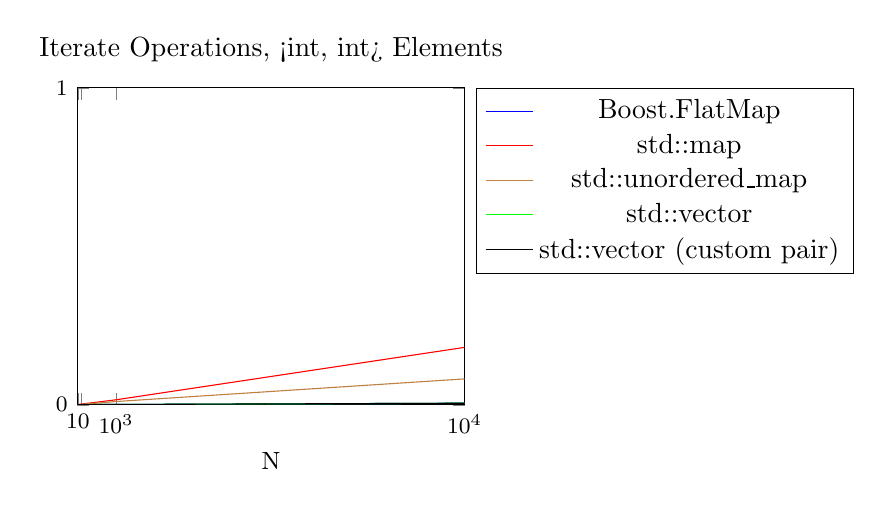
\begin{tikzpicture}[baseline]
    \begin{axis}[
        small,legend pos=outer north east,legend entries={Boost.FlatMap,std::map,std::unordered\_map,std::vector,std::vector (custom pair)},
        %width=3.75in,
        title={Iterate Operations, <int, int> Elements},
        xlabel={N},
        ylabel=\empty,%{Time [milliseconds]},
        xmin=0, xmax=10000,
        ymin=0, ymax=1.0,
        xtick={10,100,1000,10000,100000},
        xticklabels={10,,$10^{3}$,$10^{4}$,$10^{5}$},
        ytick={0.0,1.0,2.0},
        ymajorgrids=true,
        grid style=dashed,
        scaled x ticks=false,
        scaled y ticks=true,
        ]

    \addplot[color=blue,mark=|,no markers,]
        coordinates {(10,0.0006148)(100,0.0007682)(1000,0.000978)(10000,0.0049866)};

    \addplot[color=red,mark=|,no markers,]
        coordinates {(10,0.0007122)(100,0.002165)(1000,0.015826)(10000,0.181238)};

    \addplot[color=brown,mark=|,no markers,]
        coordinates {(10,0.0007266)(100,0.001299)(1000,0.0102944)(10000,0.0817004)};

    \addplot[color=green,mark=|,no markers,]
        coordinates {(10,0.0007266)(100,0.0006282)(1000,0.000978)(10000,0.0049446)};

    \addplot[color=black,mark=|,no markers,]
        coordinates {(10,0.0006286)(100,0.0006148)(1000,0.000964)(10000,0.0049028)};

    \end{axis}%
\end{tikzpicture}%
~%
%
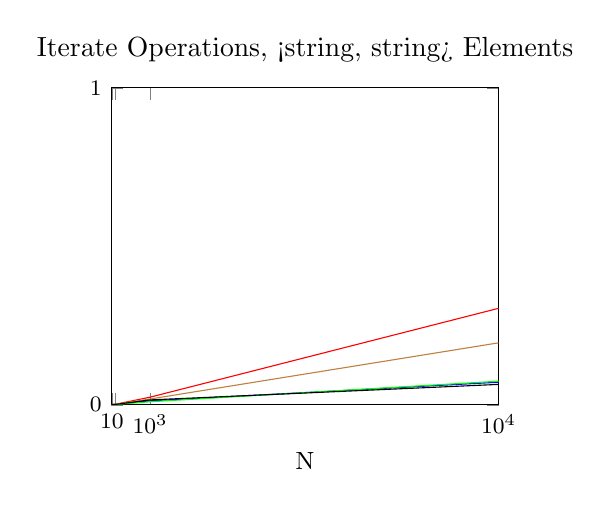
\begin{tikzpicture}[baseline]
    \begin{axis}[
        small,
        %width=3.75in,
        title={Iterate Operations, <string, string> Elements},
        xlabel={N},
        ylabel=\empty,%{Time [milliseconds]},
        xmin=0, xmax=10000,
        ymin=0, ymax=1.0,
        xtick={10,100,1000,10000,100000},
        xticklabels={10,,$10^{3}$,$10^{4}$,$10^{5}$},
        ytick={0.0,1.0,2.0},
        ymajorgrids=true,
        grid style=dashed,
        scaled x ticks=false,
        scaled y ticks=true,
        ]

    \addplot[color=blue,mark=|,no markers,]
        coordinates {(10,0.0007126)(100,0.0011034)(1000,0.0124458)(10000,0.0711818)};

    \addplot[color=red,mark=|,no markers,]
        coordinates {(10,0.0007268)(100,0.0015926)(1000,0.0240674)(10000,0.304508)};

    \addplot[color=brown,mark=|,no markers,]
        coordinates {(10,0.000629)(100,0.0012296)(1000,0.0182844)(10000,0.195542)};

    \addplot[color=green,mark=|,no markers,]
        coordinates {(10,0.0007262)(100,0.0011312)(1000,0.0095966)(10000,0.074521)};

    \addplot[color=black,mark=|,no markers,]
        coordinates {(10,0.0006708)(100,0.001118)(1000,0.0153788)(10000,0.0643378)};

    \end{axis}%
\end{tikzpicture}%
~%
%

For all variants but \code{map}, iteration is relatively similar, and much
faster that \code{map}'s.

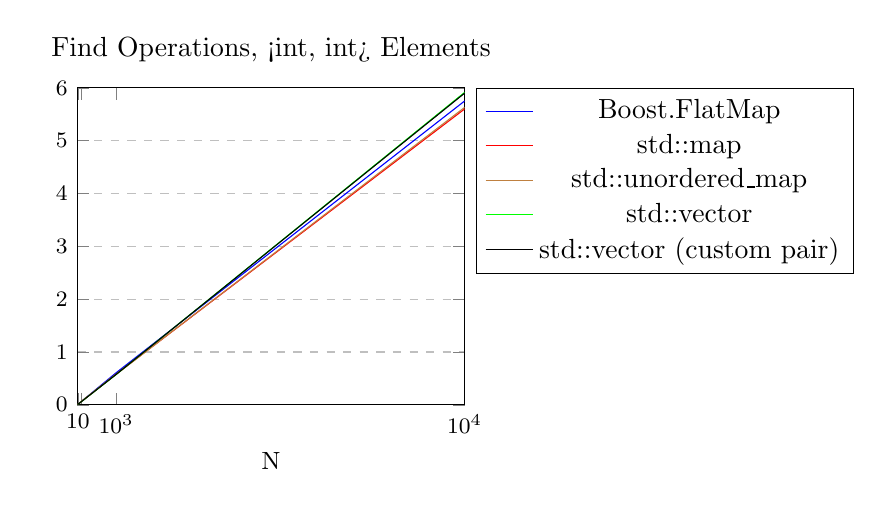
\begin{tikzpicture}[baseline]
    \begin{axis}[
        small,legend pos=outer north east,legend entries={Boost.FlatMap,std::map,std::unordered\_map,std::vector,std::vector (custom pair)},
        %width=3.75in,
        title={Find Operations, <int, int> Elements},
        xlabel={N},
        ylabel=\empty,%{Time [milliseconds]},
        xmin=0, xmax=10000,
        ymin=0, ymax=6.0,
        xtick={10,100,1000,10000,100000},
        xticklabels={10,,$10^{3}$,$10^{4}$,$10^{5}$},
        ytick={0.0,1.0,2.0,3.0,4.0,5.0,6.0,7.0},
        ymajorgrids=true,
        grid style=dashed,
        scaled x ticks=false,
        scaled y ticks=true,
        ]

    \addplot[color=blue,mark=|,no markers,]
        coordinates {(10,0.0061042)(100,0.0619778)(1000,0.60702)(10000,5.75315)};

    \addplot[color=red,mark=|,no markers,]
        coordinates {(10,0.0065656)(100,0.0617254)(1000,0.580172)(10000,5.60213)};

    \addplot[color=brown,mark=|,no markers,]
        coordinates {(10,0.0064952)(100,0.0629964)(1000,0.576962)(10000,5.63177)};

    \addplot[color=green,mark=|,no markers,]
        coordinates {(10,0.0063698)(100,0.0582888)(1000,0.573966)(10000,5.91615)};

    \addplot[color=black,mark=|,no markers,]
        coordinates {(10,0.0064248)(100,0.0581646)(1000,0.575594)(10000,5.90158)};

    \end{axis}%
\end{tikzpicture}%
~%
%
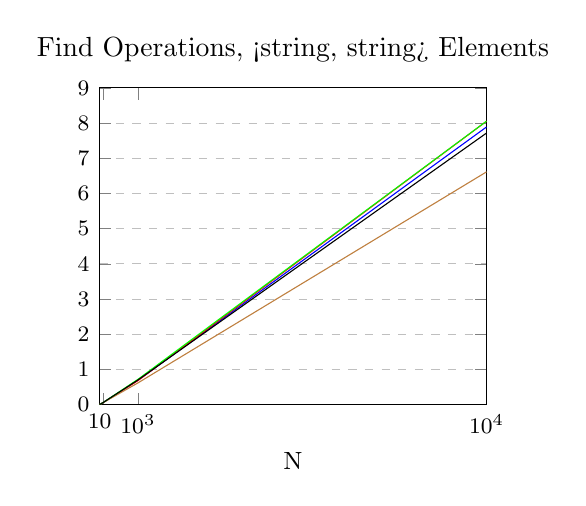
\begin{tikzpicture}[baseline]
    \begin{axis}[
        small,
        %width=3.75in,
        title={Find Operations, <string, string> Elements},
        xlabel={N},
        ylabel=\empty,%{Time [milliseconds]},
        xmin=0, xmax=10000,
        ymin=0, ymax=9.0,
        xtick={10,100,1000,10000,100000},
        xticklabels={10,,$10^{3}$,$10^{4}$,$10^{5}$},
        ytick={0.0,1.0,2.0,3.0,4.0,5.0,6.0,7.0,8.0,9.0,10.0},
        ymajorgrids=true,
        grid style=dashed,
        scaled x ticks=false,
        scaled y ticks=true,
        ]

    \addplot[color=blue,mark=|,no markers,]
        coordinates {(10,0.006118)(100,0.062631)(1000,0.695828)(10000,7.89026)};

    \addplot[color=red,mark=|,no markers,]
        coordinates {(10,0.006146)(100,0.061546)(1000,0.687874)(10000,8.05409)};

    \addplot[color=brown,mark=|,no markers,]
        coordinates {(10,0.0062576)(100,0.060553)(1000,0.621572)(10000,6.61517)};

    \addplot[color=green,mark=|,no markers,]
        coordinates {(10,0.0065508)(100,0.0637798)(1000,0.723151)(10000,8.05563)};

    \addplot[color=black,mark=|,no markers,]
        coordinates {(10,0.0064962)(100,0.063536)(1000,0.705945)(10000,7.71759)};

    \end{axis}%
\end{tikzpicture}%
~%
%

\code{find()} performance is roughly similar across all the
implementations, and they all show superlinear growth.  Note that
Boost.FlatMap performs the best here.

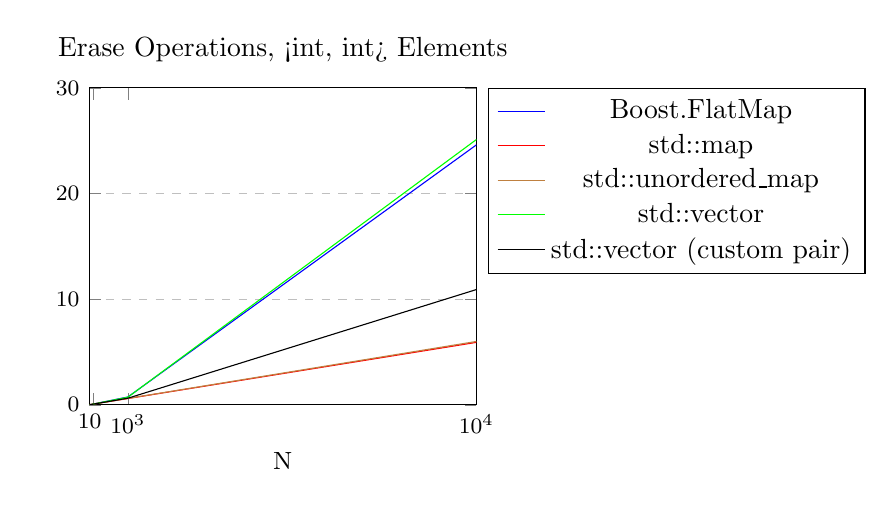
\begin{tikzpicture}[baseline]
    \begin{axis}[
        small,legend pos=outer north east,legend entries={Boost.FlatMap,std::map,std::unordered\_map,std::vector,std::vector (custom pair)},
        %width=3.75in,
        title={Erase Operations, <int, int> Elements},
        xlabel={N},
        ylabel=\empty,%{Time [milliseconds]},
        xmin=0, xmax=10000,
        ymin=0, ymax=30.0,
        xtick={10,100,1000,10000,100000},
        xticklabels={10,,$10^{3}$,$10^{4}$,$10^{5}$},
        ytick={0.0,10.0,20.0,30.0,40.0},
        ymajorgrids=true,
        grid style=dashed,
        scaled x ticks=false,
        scaled y ticks=true,
        ]

    \addplot[color=blue,mark=|,no markers,]
        coordinates {(10,0.0064952)(100,0.0667284)(1000,0.738798)(10000,24.6091)};

    \addplot[color=red,mark=|,no markers,]
        coordinates {(10,0.006774)(100,0.0651334)(1000,0.591387)(10000,5.90963)};

    \addplot[color=brown,mark=|,no markers,]
        coordinates {(10,0.0072904)(100,0.0710708)(1000,0.604785)(10000,5.99803)};

    \addplot[color=green,mark=|,no markers,]
        coordinates {(10,0.0067054)(100,0.0593234)(1000,0.724238)(10000,25.1154)};

    \addplot[color=black,mark=|,no markers,]
        coordinates {(10,0.0065508)(100,0.058947)(1000,0.624071)(10000,10.9113)};

    \end{axis}%
\end{tikzpicture}%
~%
%
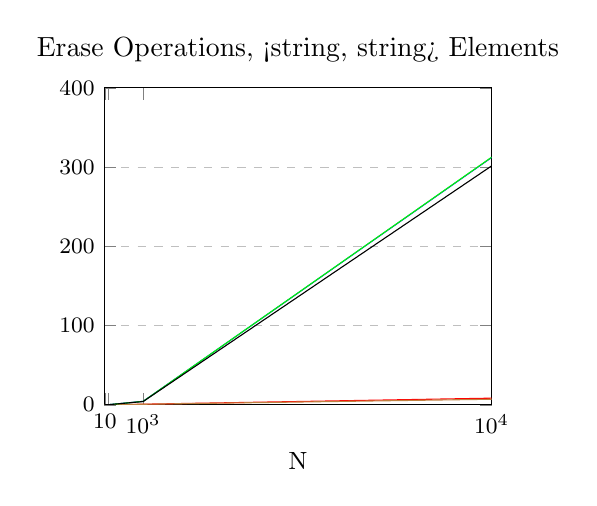
\begin{tikzpicture}[baseline]
    \begin{axis}[
        small,
        %width=3.75in,
        title={Erase Operations, <string, string> Elements},
        xlabel={N},
        ylabel=\empty,%{Time [milliseconds]},
        xmin=0, xmax=10000,
        ymin=0, ymax=400.0,
        xtick={10,100,1000,10000,100000},
        xticklabels={10,,$10^{3}$,$10^{4}$,$10^{5}$},
        ytick={0.0,100.0,200.0,300.0,400.0,500.0},
        ymajorgrids=true,
        grid style=dashed,
        scaled x ticks=false,
        scaled y ticks=true,
        ]

    \addplot[color=blue,mark=|,no markers,]
        coordinates {(10,0.0065378)(100,0.0882488)(1000,4.31769)(10000,312.192)};

    \addplot[color=red,mark=|,no markers,]
        coordinates {(10,0.006341)(100,0.0626998)(1000,0.726333)(10000,8.35754)};

    \addplot[color=brown,mark=|,no markers,]
        coordinates {(10,0.0066332)(100,0.0646158)(1000,0.666744)(10000,6.99973)};

    \addplot[color=green,mark=|,no markers,]
        coordinates {(10,0.0065636)(100,0.0885592)(1000,4.28671)(10000,312.522)};

    \addplot[color=black,mark=|,no markers,]
        coordinates {(10,0.00651)(100,0.0868132)(1000,4.09533)(10000,301.57)};

    \end{axis}%
\end{tikzpicture}%
~%
%

Erasure has a similar performance profile to insertion, except that the sorted
\code{vector<pair<int, int>>} performs substantially better than
Boost.FlatMap.\\


\subsection{Implications}

TODO Iteration is vastly cheaper for contiguous-storage variants.  It has been
suggested that a \code{map} with a custom allocator can achieve similar
performance to flat data structures, but this would not apply to iteration
performance, unless the values were added to the \code{map} in sorted order.\\

In all the graphs above, the reason the custom-\code{pair} sorted vector
performs so much better than \code{vector<pair<int, int>>} seems to be that
the custom-\code{pair} type has \code{nothrow} special functions.
Implementing all the special functions and adding \code{nothrow(false)} to
each makes the custom-\code{pair} version perform identically to the
\code{pair<int, int>} version.

Boost.FlatMap differs quite a bit from a sorted \code{vector}.  Clearly there
are a lot of QOI choices to make in implementing a standard \code{flat_map}.
